\chapter{Vector Geometry}
\label{Chapter:02vectors}
 
Much of the material in this chapter may be review from high
school, but it allows us to set the stage 
 for the upcoming chapters.



\section{Vectors in \texorpdfstring{$\R^n$}{Rn}}

\stress{Vector} comes from the Latin \textit{vehere}, which means to carry,
or to convey; abstractly we think of the vector as taking us along the
arrow that we represent it with.  For example, we use vectors in Physics to indicate the magnitude and direction of a
force.

Let's use our understanding of the geometry and algebra of vectors in
low dimensions (2 and 3) to develop some ideas about the geometry and
algebra in higher dimensions.

\begin{center}
\begin{tabular}{ll}
Algebra & Geometry \\
\hline
$\R$, real numbers, \defn{scalars} & real line\\
$\R^2 = \{(x,y) | x,y\in\R\}$, vectors $\uu = (x,y)$ & plane \\
$\R^3 = \{(x,y,z) | x,y,z\in\R\}$, vectors $\uu = (x,y,z)$ & 3-space \\
\vdots & \\
(why not keep going?) & \\
\vdots & \\
$\R^4 = \{(x_1,x_2,x_3,x_4) | x_i \in \R\}$, vectors $\xx = (x_1,x_2,x_3,x_4)$ & \\
Hamilton (1843): extended $\C$ to \defn{hamiltonians} & \defn{space-time}\\
& \\
$n \in \Z$, $n>0$: $\R^n = \{ (x_1, x_2,\cdots,x_n) | x_i \in \R\}$ &\\
$\xx = (x_1, \cdots, x_n)$ & $n$-space
\end{tabular}
\end{center}

\paragraph{Notation}  We have several different notations which we use for
writing vectors, which we use interchangeably:
\begin{itemize}
\item $\xx = (1,2,3,4)$
\item $\xx = \mat{1\\2\\3\\4}$
\item $\xx = \mat{1\;&2\;&3\;&4}^T$, where the exponent T stands for
\defn{tranpose}.  (\emph{Transposition}\index{transposition} means turning rows into columns (and \emph{vice versa}).)
\end{itemize}
The vertical notation (also referred to as \defn{matrix form}) is the easiest to read but the first one is easier
to write.

  

(The reason for the vertical
vector notation comes from matrix multiplication, which we'll get to later.)

\section{Manipulation of vectors in \texorpdfstring{$\R^n$}{Rn}}  

The algebraic rules for $\R^n$ extend directly from the algebraic
rules for $\R^2$ and $\R^3$: 
\begin{itemize}
\item Equality:  $(x_1,\cdots, x_n) = (y_1,\cdots, y_n) \Leftrightarrow x_i=y_i$ for all $i \in \{1,\cdots,n\}$.  (In particular, $(x_1,\cdots,x_n) \neq (y_1,\cdots, y_m)$ if $n \neq m$.)

\item Addition:  $(x_1,\cdots,x_n) + (y_1,\cdots, y_n) = (x_1+y_1, \cdots, x_n+y_n)$
\item Zero vector:  $\zero = (0,0,\cdots, 0) \in \R^n$
\item Negative:  if $\xx = (x_1,\cdots,x_n)$ then $-\xx = (-x_1,\cdots,-x_n)$
\item Multiplication {\bf by a scalar}:  let $c\in \R$ be a scalar, then
$c(x_1,\cdots,x_n) = (cx_1,\cdots,cx_n)$
\end{itemize}
Note that we don't have any way of \stress{multiplying} two vectors; the closest
we can get to that is the \stress{dot product}, which gives a scalar as an 
answer, or the \stress{cross product}, which only works in $\R^3$\footnote{However, there are ways generalize the cross product in $\R^n$ for every $n$, but the product doesn't live in $\R^n$! Search the web for `exterior algebra'.}.
 There's even a way to have `multi-products' of $n-1$ vectors in $\R^n$, and get an answer in $\R^n$. Once you've seen the {\it determinant} later, you'll know exactly what to do if you look again at the definition of the cross product.

There are geometric interpretations of each of the above algebraic
rules, which we can draw in $2$ (and $3$, if you draw well) dimensions.
\begin{itemize}
\item Equality:  two vectors are equal if they have the same magnitude
and direction
\item Addition:  parallelogram rule, or head-to-tail rule 

\item Zero vector:  the vector with zero length
\item Negative: the same arrow with head and tail exchanged
\item Scalar multiple:  scale the vector by $\vert c \vert$, and change
direction if $c<0$; or:  two vectors are \emph{parallel} if and only if 
they are scalar multiples of one another.
\end{itemize}

\section{Linear combinations (Important Concept!)}
The only operations we have are:  vector addition, and scalar multiplication.
We are going to be interested in the question:  If I already have the
vectors $\uu_1$, $\uu_2$, $\cdots$, $\uu_m$ (that is, $m$
vectors in $\R^n$), can I produce another  vector 
by scaling each vector and adding them together, in some way?

By analogy:  Say $\uu_1$ is parallel to Bank Street pointing north 
and $\uu_2$
is parallel to Laurier Ave, pointing east; then I can get anywhere downtown by 
going in the direction of $\uu_1$ (or its negative) 
for a little way, and then taking direction $\uu_2$ (or its
negative) for a little way.  But I can't get underground, or
into the air, by following those directions.  I'm stuck on the
plane which is the ground.

Algebraically, this all comes down to the following definition.

\begin{definition} \index{linear combination}
If $k_1,k_2,\cdots, k_m \in \R$ are scalars, and $\uu_1,\uu_2,\cdots,\uu_m\in \R^n$ are vectors, then 
$$
k_1\uu_1+k_2\uu_2 + \cdots + k_m\uu_m 
$$
is called a \emph{linear combination} of $\uu_1,\uu_2,\cdots,\uu_m$.
\end{definition}

\begin{myexample}
Let $\uu_1 = (1,2,3)$ and $\uu_2 = (1,0,0)$.  

Then $\xx = (17,4,6)$ is a linear combination of $\uu_1$
and $\uu_2$ because
$$
\mat{17\\4\\6} = 2 \mat{1\\2\\3} + 15 \mat{1\\0\\0}.
$$
But $\yy = (0,1,0)$ is \emph{not} a linear combination of
$\uu_1$ and $\uu_2$ because the equation
\begin{equation} \label{E:1}
\mat{0\\1\\0} = a \mat{1\\2\\3} + b\mat{1\\0\\0}
\end{equation}
would imply 
\begin{align*}
\mat{0\\1\\0} &= \mat{a\\2a\\3a} + \mat{b\\0\\0}\\
&= \mat{a+b\\ 2a \\ 3a}
\end{align*}
So that
$$
0 = a+b, \quad  1 = 2a, \quad \text{and} \quad 0 = 3a;
$$ 
but the second and third equations are contradictory, so
there cannot be a solution to \eqref{E:1}.  Thus $\yy$
isn't a linear combination of $\uu_1$ and $\uu_2$.
\end{myexample}

\section{Properties of vector addition and scalar multiplication}



Note that all the usual algebraic properties of addition and
scalar multiplication hold, whether our vectors have $2$
components or $n$ components.  That is, let $\uu,\vv,\ww\in\R^n$
and let $c,c' \in \R$; then we have:
\begin{itemize}
\item $\uu+\zero = \uu$
\item $\uu + (-\uu) = \zero$
\item $(\uu + \vv) + \ww = \uu + (\vv+\ww)$

\item $\uu+\vv = \vv+\uu$
\item $c(\uu+\vv) = c\uu + c\vv$
\item $(c+c')\uu = c\uu + c'\uu$
\item $(cc')\uu = c(c'\uu)$
\item $1 \uu = \uu$
\end{itemize}
Bear these properties in mind, as they are the key to generalizing
to vector spaces beyond $\R^n$.

\section{More geometry: the Dot Product in \texorpdfstring{$\R^n$}{Rn}}  

The \defn{dot product} (also called an \defn{inner product}) gives us
an algebraic way to describe some interesting geometric properties:
length of a vector, and angle between two vectors.

Recall the dot product from $\R^3$:

Let $\uu = (x_1,x_2,x_3)$ and $\vv = (y_1,y_2,y_3)$ be two vectors in
$\R^3$.  Then their dot product is
$$
\uu \cdot \vv = x_1y_1 + x_2y_2 + x_3y_3.
$$
Note that this is a scalar.

Once we have the dot product, we define:
\begin{itemize}
\item $\Vert \uu \Vert = \sqrt{x_1^2+x_2^2+ x_3^2} = \sqrt{\uu \cdot \uu}$, the \emph{length} or \emph{norm} of $\uu$;
\item $\Vert \uu - \vv \Vert$ is the \emph{distance between $\uu$ and $\vv$}.
\end{itemize}
We can see that this is correct, by drawing a cube with main diagonal $\uu$
and noting that the length of the main diagonal is given by the square
root of the sum of the squares of the lengths of the sides by repeated
applications of the Pythagorean theorem.

So, let's generalize this to $\R^n$:

\begin{definition}
Let $\uu = (x_1,\ldots,x_n)$ and $\vv = (y_1,\ldots,y_n)$ be vectors
in $\R^n$.  Then their \defn{dot product} is defined to be 
$$
\uu \cdot \vv = x_1y_1 + \cdots + x_ny_n
$$
and the \defn{norm} of $\uu$ is defined to be
$$
\Vert \uu \Vert = \sqrt{\uu \cdot \uu} = \sqrt{x_1^2+\cdots+x_n^2}
$$
We sometimes call $\R^n$, equipped with the dot product, \defn{Euclidean
$n$-space}.\footnote{As opposed to, for example, 'Minkowski spacetime', where the `lengths' of vectors can be imaginary! Search the web for `minkowski space wiki'.}
\end{definition}


\begin{myexample}
Let $\uu = (1,2,-1,0,1)$, $\vv = (1,3,2,1,1)$.  Then
$$
\uu \cdot \vv = 1+6-2+0+1 = 6
$$
and
$\Vert \vv \Vert = \sqrt{1+9+4+1+1} = \sqrt{16}=4$.
\end{myexample}

Note that for any vector $\uu \in \R^n$:
$$
\Vert \uu \Vert = 0 \Leftrightarrow \uu = \zero
$$
(because the norm is still the sum of real squares, and so
is never zero unless each component is).

\section{Orthogonality}

Recall that in $\R^2$ and $\R^3$, we have that
$$
\uu \cdot \vv = 0 \Leftrightarrow \textrm{$\uu$ and $\vv$ are orthogonal ( or `perpendicular').}
$$

\begin{definition}
Let $\uu,\vv \in \R^n$.  Then $\uu$ and $\vv$ are said to be
\defn{orthogonal} if $\uu \cdot \vv = 0$.
\end{definition}

\begin{myexample}
The vectors $(1,2,-2,1)$ and $(4,1,3,0)$ of $\R^4$ are orthogonal
(perpendicular), since
$$
\mat{1\\2\\-2\\1} \cdot \mat{4\\1\\3\\0} = 4+2-6+0 = 0.
$$
\vglue -.5cm
\end{myexample}

\section{Angles between vectors in \texorpdfstring{$\R^n$}{Rn}}

Now saying that two vectors are orthogonal is another way of
saying that they meet at a $90^\circ$ angle.  We can determine
the angle between vectors in $\R^2$ and $\R^3$; can that be
generalized as well?  We need to know one fact:


\begin{theorem}[Cauchy-Schwarz Inequality]
If $\uu,\vv \in \R^n$, then 
$$
\vert \uu \cdot \vv \vert \leq \Vert \uu \Vert \; \Vert \vv \Vert
$$
\end{theorem}

The proof\footnote{For $x\in\R$, consider the   quadratic function $q(x)=\|u+ x v\|^2$. Expand the right hand side as $(u+ x v)\cdot (u+ x v)$, compute the discriminant `$b^2-4ac$', which (as $q(x)\ge 0$ for all $x$) must satisfy $b^2-4ac\le 0$. Simplifying this, one obtains the desired inequality.} is straightforward.

Applying this to $\Vert \uu + \vv \Vert^2 = (\uu + \vv)\cdot(\uu+\vv)$
yields
$$
\Vert \uu + \vv \Vert \leq \Vert \uu \Vert + \Vert \vv \Vert
$$
which is the \defn{triangle inequality} (which looks the same as the one we noted for $\C$
in our first class).

\begin{definition}
If $\uu,\vv \in \R^n$ and $\uu,\vv \neq \zero$, then the angle
$\theta$ between $\uu$ and $\vv$ is defined to be the number
$\theta$ which satisfies:
\begin{itemize}
\item $\displaystyle \cos \theta = \frac{\uu \cdot \vv}{\Vert \uu \Vert\; \Vert \vv \Vert}$
\item $0 \leq \theta \leq \pi$
\end{itemize}
(The first condition makes sense because
of the Cauchy-Schwarz inequality, since this inequality implies that the number on the right hand
side is always between $-1$ and $1$. The second condition guarantees uniqueness of $\theta$. )
\end{definition}

\begin{myexample}
The angle between $\uu = (0,0,3,4,5)$ and $\vv = (-1,1,-1,1,2)$
is $\theta$, where
$$
\cos(\theta) = \frac{\uu \cdot \vv}{\Vert \uu \Vert\; \Vert \vv \Vert}
= \frac{11}{\sqrt{50}\sqrt{8}} = \frac{11}{20}.
$$
 We find $\theta = \arccos(11/20)$.\footnote{With the help of a calculator --which you'll never need in this course --, $\theta \simeq 0.988432\simeq56.6^\circ$.}
\end{myexample}

Of particular interest:
\begin{itemize}
\item Two non-zero vectors $\uu$, $\vv$ are orthogonal if the angle between
them is $\frac{\pi}2$ (or $90^\circ$).  Now $\cos(\frac{\pi}2) = 0$, so by our formula,
the numerator $\uu \cdot \vv$ has to be zero.  That's where the
orthogonality condition came from.
\item Two vectors $\uu$ and $\vv$ are parallel if the angle between
them is either $0^\circ$ or $\pi$.  Now $\cos(0) = 1$ and
$\cos(\pi) = -1$, so in this case $\uu \cdot \vv = \pm \Vert \uu \Vert\; \Vert \vv \Vert$ attains its maximum value (in absolute terms).
\end{itemize}

\section{Orthogonal Projections onto lines in \texorpdfstring{$\R^n$}{Rn}}
 
The idea of the 
orthogonal projection is:  given two nonzero vectors $\uu$ and $\vv$,
then the \defn{projection of $\vv$ onto $\uu$}, denoted

  
$$
 \proj_{\uu}(\vv)
$$ 
is the unique vector which satisfies
\begin{itemize}\label{propOrthogProj}
\item $\proj_{\uu}(\vv)$ is parallel to  
$\uu$ (so a scalar multiple of $\uu$)
\item $\vv - \proj_{\uu}(\vv)$ is orthogonal to $\uu$ (so gives dot product zero).
\end{itemize}
 
\begin{figure}
\begin{center}
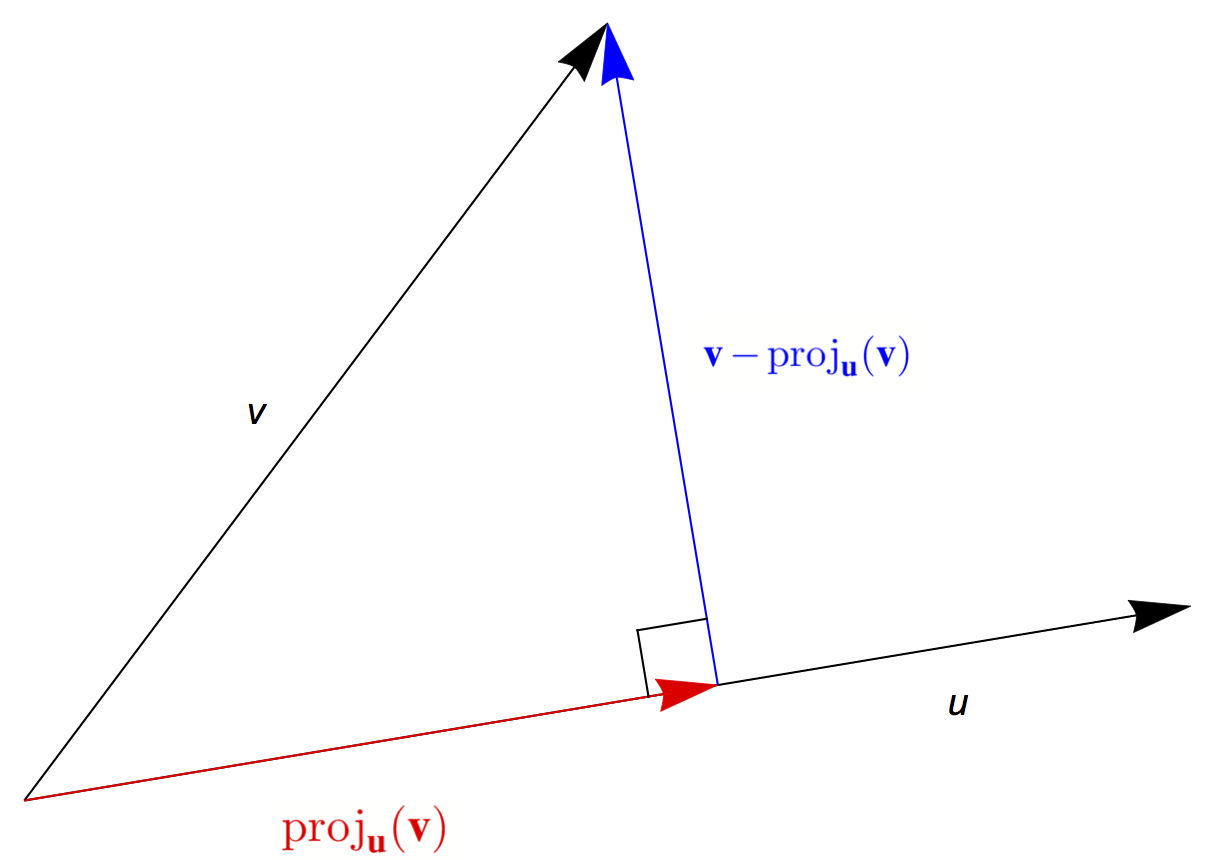
\includegraphics[width=3in]{img/decomp.jpg}
\end{center}
\caption{Orthogonal projection of $\vv$ on $\uu$.}\label{orthoprojonvector}
\end{figure}
As a result, we have \stress{decomposed} $\vv$ as a sum
$$
\vv = (\proj_{\uu}(\vv))+ (\vv-\proj_{\uu}(\vv))
$$
of something parallel to $\uu$ and something perpendicular to $\uu$,
as in our picture.

So how do we find $\proj_{\uu}(\vv)$?  It turns out to be easy.
Using either trigonometry, or just solving directly from the above
two conditions, you get:
$$
\proj_{\uu}(\vv) = \frac{\vv \cdot \uu}{\Vert \uu \Vert^2} \uu.
$$\label{projR3}
(Careful: the quotient is just a scalar.  To remember this:
if you are projecting
onto $\uu$ your answer is always a multiple of $\uu$, which is
also the term that appears in the denominator.) 

\begin{myexample}
Let $\uu = (1,0,0)$ and $\vv = (2,3,4)$.  Write $\vv$ as a sum
of two vectors, one parallel to $\uu$ and one orthogonal to $\uu$.
(Presumably you could guess the answer to this one, but let's
see what the formula does.)  We calculate:
$$
\proj_{\uu}(\vv) = \frac{\vv \cdot \uu}{\Vert \uu \Vert^2} \uu
= \frac{2+0+0}{1^2+0^2+0^2}\mat{1\\0\\0} = \mat{2\\0\\0}
$$
and $\vv - \proj_{\uu}(\vv) = (2,3,4)-(2,0,0) = (0,3,4)$, so our
decomposition is
$$
\vv = \mat{2\\3\\4} = \mat{2\\0\\0}+\mat{0\\3\\4}
$$
and it's clear that the first is parallel to $\uu$ while the 
second is orthogonal to $\uu$ --- and that this is the only
possible pair of vectors that satisfy this.
\end{myexample}

\begin{myexample}
Let $\uu = (1,1)$ and $\vv = (2,3)$.  Then
$$
\proj_{\uu}(\vv) = \frac{\vv \cdot \uu}{\Vert \uu \Vert^2} \uu
= \frac{2+3}{1^2+1^2}\mat{1\\1} = \mat{5/2\\ 5/2}
$$
is the projection of $(2,3)$ onto $(1,1)$.
\end{myexample}

Orthogonal projection is used in UMTS (Universal Mobile Telecommunications System) to correct fuzziness and errors in signals and produce more reliable
communications.

Another way of talking about orthogonal projection is to say that
we are finding the closest point to $\vv$ on the line from the origin in
direction $\uu$.  So our next goal is to talk about lines and planes.


